\textbf{See the instruction for questions \inteval{\value{question}+1} to \inteval{\value{question}+2}.}

\begin{figure}[H]
    \centering
    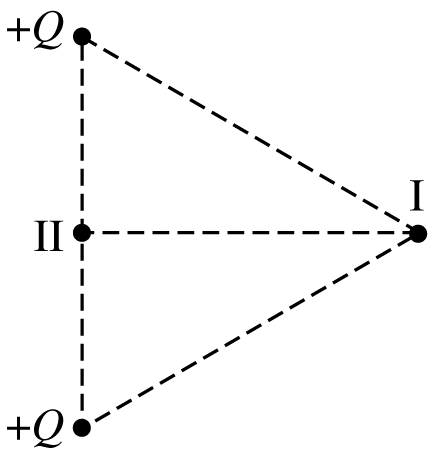
\includegraphics[scale=0.3]{images/img-002-000.png}
\end{figure}

In the figure above, two small spheres, each with charge $+Q$, are fixed in place at the corners of an equilateral triangle. Point $\mathrm{I}$ is at the third corner, and point II is midway between the charges.

% Multiple Choice Question 1
\begin{questions}\setcounter{question}{0}\question
A small particle with charge $+q$, where $q \ll Q$, is moved from point I to point II at constant speed $v$ by an external force. $W_\mathrm{EXT}$ is the work done by the external force on the moving charge, and $W_\mathrm{ELEC}$ is the work done by the electrostatic force. Which of the following correctly identifies the signs of these quantities?

\tabto{0.75cm}\underline{$W_\mathrm{EXT}$}
\tabto{3.00cm}\underline{$W_\mathrm{ELEC}$}

\begin{choices}
\choice $+$ \tabto{2.25cm} $+$
\choice $+$ \tabto{2.25cm} $-$
\choice $-$ \tabto{2.25cm} $+$
\choice $-$ \tabto{2.25cm} $-$
\choice None of the above, since the work done by both the external force and the electrostatic force is zero.
\end{choices}\end{questions}

% Multiple Choice Question 2
\begin{questions}\setcounter{question}{1}\question
Which of the following best describes the relationship between the electric potentials $V_\mathrm{I}$ and $V_\mathrm{II}$ at points I and II, respectively?

\begin{choices}
\choice $V_\mathrm{I} < V_\mathrm{II}$
\choice $V_\mathrm{I} = V_\mathrm{II}$
\choice $V_\mathrm{I} > V_\mathrm{II}$
\choice It cannot be determined without knowing the magnitudes of the charges.
\choice It cannot be determined without knowing the distance between points I and II.
\end{choices}\end{questions}
